The existence of gravitational waves is a direct consequence of Einstein's theory of general relativity (GR), which describes gravity in terms of the differential geometry of curved spacetime. The theory states that the presence of matter causes a curvature of spacetime and particles move along the shortest path in this curved space, along so-called \emph{geodesics}.
This chapter provides a brief introduction to general relativity and how gravitational waves emerge from this theory. It discusses their properties and astrophysical sources, focusing on compact binary systems since these are the only type of signals considered in this work. The sources for this chapter are \cite{10.1093/acprof:oso/9780198570745.001.0001} and to a lesser extent \cite{Carroll_2004}. 

\section{General Relativity}

%\begin{figure}
%	\centering
%	\makebox[\textwidth]{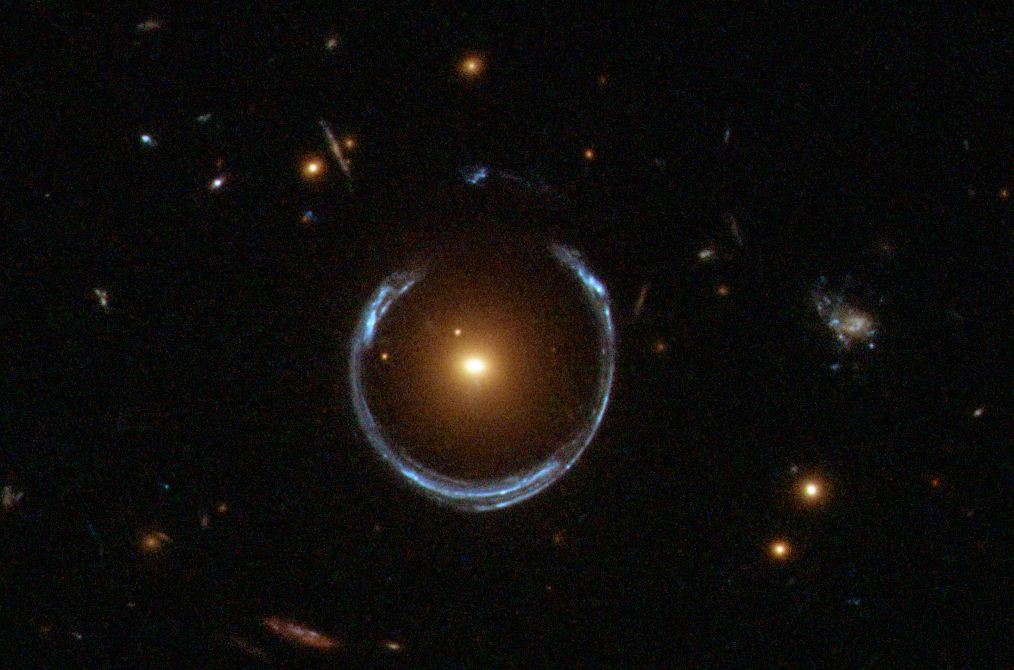
\includegraphics[width=5cm]{theory_of_gravitational_waves/images/A_Horseshoe_Einstein_Ring_from_Hubble}}
%	\caption{}
%	\label{fig:gravitational_waves:lensing}
%\end{figure}	

The theory of general relativity is based on the \emph{strong equivalence principle}, which states that there is no way to distinguish free-falling frames from one another by performing local experiments and that locally, \emph{special relativity} holds. This postulate alone gives rise to effects such as gravitational redshift or the bending of light near large masses. The equivalence principle then leads to a four-dimensional geometric description of spacetime, which is based on the metric tensor $g_{\mu\nu}$ whose indices denote the time and spatial axes, $t$, $x$, $y$ and $z$.
The metric tensor defines local distances in curved spacetime which are invariant under coordinate transformations through the differential line element,
\begin{equation}
	\label{eq:gravitational_waves:line_element}
	\mathrm{d}s^2 = g_{\mu\nu}\mathrm{d}x^\mu\mathrm{d}x^\nu
\end{equation}
with $x^\mu = (ct, \vec{r})$ where $c$ is the speed of light.
This is a generalization from the invariant quadratic form in special relativity, where
spacetime is flat. Then, the metric tensor is the \emph{Minkowski} metric $\eta_{\mu\nu} = \diag(-1, 1, 1, 1)$ and Eq.~\ref{eq:gravitational_waves:line_element} reads 
\begin{equation}
	\mathrm{d}s^2 = -c^2\mathrm{d}t^2 + \mathrm{d}x^2 + \mathrm{d}y^2 + \mathrm{d}z^2.
\end{equation}

The equations of motion for the metric $g_{\mu\nu}$ can be derived by defining the gravitational action, which depends on the metric itself and the matter content. Then, by requiring that the variation of this action with respect to the metric be zero, one arrives at the \emph{Einstein equations},
\begin{equation}
	\label{eq:gravitational_waves:einstein_eqs}
	R_{\mu\nu} - \frac{1}{2}Rg_{\mu\nu} = \frac{8\pi G}{c^4}T_{\mu\nu}.
\end{equation}
These equate the \emph{energy-momentum tensor} $T_{\mu\nu}$ with the \emph{Einstein tensor} $G_{\mu\nu} = R_{\mu\nu} - Rg_{\mu\nu}/2$ on the left-hand side up to some constant, where $G$ is Newton's constant. The energy-momentum tensor describes the matter and energy content and the Einstein tensor expresses the resulting spacetime curvature. The latter is constructed from the metric $g_{\mu\nu}$ as well as the \emph{Ricci tensor} $R_{\mu\nu}$ and the \emph{Ricci scalar} $R$, both of which also depend on the metric through various partial derivatives and index contractions. 

Without any forces acting, particle trajectories will follow geodesics of this curved spacetime.
Knowing the spacetime curvature, these can be calculated using the \emph{geodesic equation},
\begin{equation}
	\label{eq:gravitational_waves:geodesic_eq}
	\frac{\mathrm{d}^2x^\lambda}{\mathrm{d}\tau^2} 
	+ \Gamma^\lambda_{\mu\nu}\,
	\frac{\mathrm{d}x^\mu}{\mathrm{d}\tau}\,
	\frac{\mathrm{d}x^\nu}{\mathrm{d}\tau}
	= 0
\end{equation}
where $\tau$ is the particle's proper time and $\Gamma^\lambda_{\mu\nu}$ denote the \emph{Christoffel symbols} which depend on the curvature. 
% what is proper time? the time the particle measures along its trajectory that is in its reference frame which is at rest ds = c dtau

It can be seen that GWs naturally emerge from GR when working in \emph{linearized theory}: The GW's effect on spacetime is thought of as a \enquote{small} perturbation $h_{\mu\nu}$ of flat spacetime. Then, spacetime can be expanded as
\begin{equation}
	\label{eq:gravitational_waves:linearized_theory}
	g_{\mu\nu} = \eta_{\mu\nu} + h_{\mu\nu} \quad\text{with $|h_{\mu\nu}|\ll1$},
\end{equation}
and any terms of higher order than $\pazocal{O}(h_{\mu\nu})$ are neglected in following calculations. Further simplifications can be made by noting that
GR is invariant under \emph{all possible} coordinate transformations. This corresponds to large number of degrees of freedom, \emph{i.e.}, a large \emph{gauge symmetry}. 
Imposing linearized theory breaks that invariance, but still a residual gauge symmetry remains. 
% this is sloppy and wrong maybe?
Thus, the \emph{Lorenz gauge} can be chosen, $\partial^\mu\bar{h}_{\mu\nu} = 0$. Then the Einstein equations (Eq.~\ref{eq:gravitational_waves:einstein_eqs}) simply reduce to wave equations,
\begin{equation}
	\label{eq:gravitational_waves:wave_eq}
	\square\,\bar{h}_{\mu\nu} = -\frac{16\pi G}{c^4}\,T_{\mu\nu}
\end{equation}
with the d'Alembertian $\square=\partial_\mu\partial^\mu=-\partial_t^2/c^2 + \nabla^2$.\footnote{Indices are raised and lowered using the Minkowski metric in linearized theory.}
Here, $\bar{h}_{\mu\nu}$ denotes the \emph{trace-reversed} perturbation, which is defined as
\begin{equation}
	\bar{h}_{\mu\nu} = h_{\mu\nu}-\frac{1}{2}\eta_{\mu\nu}h,
\end{equation}
where $h = \eta^{\mu\nu}h_{\mu\nu}$ is the original perturbation's trace. The trace-reversed perturbation gets its name from the fact that its trace $\bar{h} = \eta^{\mu\nu}\bar{h}_{\mu\nu} = -h$. Obviously, the original perturbation can be reconstructed from the trace-reversed one, so no information is lost. 
Eq.~\ref{eq:gravitational_waves:wave_eq} shows that GWs obey an inhomogeneous wave equation with the matter content $T_{\mu\nu}$ as its source. 

\section{Properties in Vacuum}

To study the propagation of GWs and their influence on nearby particles (also called test masses in this context) it makes sense to consider the case far away from the sources that produce them. This is called the \emph{vacuum case}, where $T_{\mu\nu} = 0$.
The Einstein equations (Eq.~\ref{eq:gravitational_waves:wave_eq}) now read,
\begin{equation}
	\label{eq:gravitational_waves:homogeneous_wave_eq}
	\square\,\bar{h}_{\mu\nu} = 0.
\end{equation}
These equations have plane-wave solutions, 
\begin{equation}
	\bar{h}_{\mu\nu} = A_{\mu\nu}\,\e^{ik_\rho x^\rho}
\end{equation}
with a wave-vector $k^\mu = (\omega/c, \vec{k})$ and some constant amplitude $A_{\mu\nu}$. This introduces complex numbers, and only the real part is considered at the end of calculations. For the plane-wave solutions, the Einstein equations (Eq.~\ref{eq:gravitational_waves:homogeneous_wave_eq}) imply that $k_\mu k^\mu = 0$, which loosely translates to the fact that GWs propagate at the speed of light. The Lorenz gauge condition yields $A^{\mu\nu}k_\mu=0$, \emph{i.e.}, the amplitude and wave-vector are orthogonal.

Now for reasons that will not be laid out here, the vacuum case allows for the introduction of the \emph{transverse-traceless} gauge with
\begin{equation}
	h^{0\mu} = 0 \quad \text{and} \quad h^i_{\phantom{i}i} = 0,
\end{equation}
where Latin indices, such as $i,j,k$, denote spatial components only. For further information, consult \cite{10.1093/acprof:oso/9780198570745.001.0001}. In this gauge the trace $h$ vanishes and thus $\bar{h}_{\mu\nu} = h_{\mu\nu}$. The Lorenz condition then reads $A^{ij}k_j=0$: GWs are transverse, meaning they perturb the metric orthogonal to their propagation direction.

\begin{figure}
	\centering
	\makebox[\textwidth]{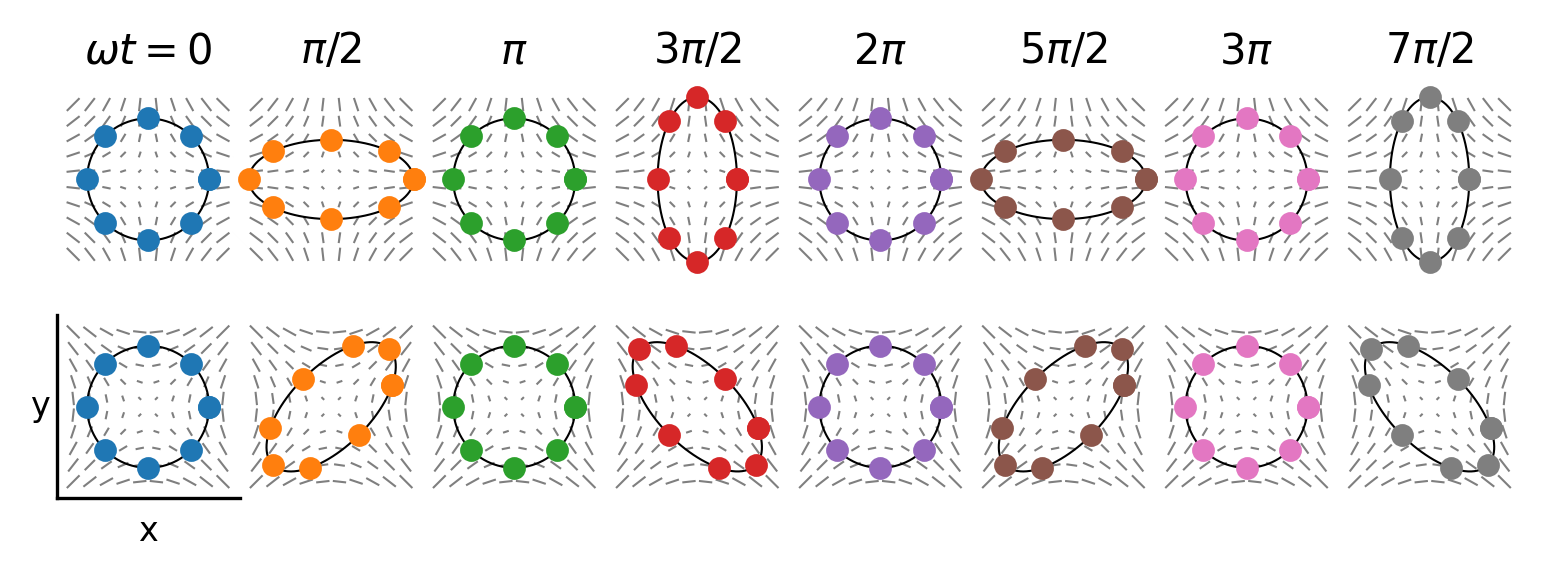
\includegraphics[width=16cm]{theory_of_gravitational_waves/images/test_masses/polarization_trajectories}}
	\caption{The effect of a passing GW on a ring of test masses on the transverse plane. The top row shows a purely plus-polarized GW, and the bottom row a cross-polarized one.}
	\label{fig:gravitational_waves:polarization}
\end{figure}

To illustrate their effect on test masses, one can arbitrarily choose a GW to propagate along the z-axis, $\vec{k}=(0,0,\omega/c)$. Enforcing the gauge conditions, only two components of the amplitude remain and the GW perturbation takes the following form:
\begin{equation}
	h_{\mu\nu} = \begin{pmatrix}
		0 & 0 & 0 & 0 \\
		0 & A_+ & A_\times & 0 \\
		0 & A_\times & -A_+ & 0 \\
		0 & 0 & 0 & 0
	\end{pmatrix}_{\mu\nu} \e^{i\omega(t-\frac{z}{c})} = h_+e_{\mu\nu}^+ + h_\times e_{\mu\nu}^\times
\end{equation}
with $h_+ = A_+\exp i\omega(t-z/c)$ and $h_\times = A_\times\exp i\omega(t-z/c)$.
The result is split along two linearly independent polarizations, labeled \emph{plus} (\text{$+$}) and \emph{cross} (\text{$\times$}). Each is described by a polarization tensor, $e_{\mu\nu}^+$ and $e_{\mu\nu}^\times$, which are orthogonal, $e_{\mu\nu}^+e^\times{}^{\mu\nu} = 0$. The plus and cross polarization states get their names from their effect on nearby test masses.

The trajectories of nearby particles with separation vectors $S^\mu$ follow from the geodesic equation (\ref{eq:gravitational_waves:geodesic_eq}). It can be seen that the test masses are only perturbed perpendicular to the GW's propagation direction in the x--y plane. In particular, solving for a purely plus-polarized wave, $h_\times=0$, yields
\begin{equation}
	\label{eq:gravitational_waves:plus_polarization}
	\begin{aligned}
		S^1 &= S^1(0) + \frac{h_+}{2}\,S^1(0), \quad
		S^2 &= S^2(0) - \frac{h_+}{2}\,S^2(0).
	\end{aligned}
\end{equation}
Thus, particles initially separated on the x-axis will oscillate in that same direction; likewise for particles on the y-axis but with a phase shift of \SI{180}{\degree}. Considering a ring of test particles around the origin, one can see that they oscillate in a plus-shaped manner.
Now, in the case that the GW is purely cross-polarized, $h_+=0$ and $h_\times\neq0$, the solution is instead given by
\begin{equation}
\label{eq:gravitational_waves:cross_polarization}
\begin{aligned}
	S^1 &= S^1(0) + \frac{h_\times}{2}\,S^2(0), \quad
	S^2 &= S^2(0) - \frac{h_\times}{2}\,S^1(0),
\end{aligned}
\end{equation}
and a ring of test masses will oscillate cross-wise.
The effect of these two polarization states can be seen plotted in Fig.~\ref{fig:gravitational_waves:polarization}.

\section{Production}
\label{sec:gravitational_waves:production}

Having studied their properties in the vacuum case, one can now take one step back and consider the production of GWs. This means considering $T_{\mu\nu} \neq 0$ (where now only the Lorenz gauge and \emph{not} the transverse-traceless gauge can be chosen), in which case the Einstein equations take the form of an inhomogeneous wave equation again, $\square\,\bar{h}_{\mu\nu} = -(16\pi G/c^4)\,T_{\mu\nu}$ (see Eq.~\ref{eq:gravitational_waves:wave_eq}). The solutions to this equation are known:
\begin{equation}
	\bar{h}_{\mu\nu} = \frac{4G}{c^4} 
	\int\mathrm{d}^3\vec{r}'\, 
	\frac{T_{\mu\nu}\bigl(t-\frac{|\vec{r}-\vec{r}'|}{c}, \vec{r}'\bigr)}
	{|\vec{r}-\vec{r}'|}.
\end{equation}
That is, the GW perturbation observed at position $(t, \vec{r})$ is caused by the sum of all sources $T_{\mu\nu}$ evaluated at time $t_\text{ret} = t-|\vec{r}-\vec{r}'|/c$, the \emph{retarded time}. (If a source at $\vec{r}'$ emits a signal at time $t_\text{ret}$ it will reach the observer position $\vec{r}$ at time $t$.) Making the assumption that the source volume is \enquote{small} and that it is far away from the observer allows approximating the distance between the two as $|\vec{r}-\vec{r}'| \approx |\vec{r}| = r$.
Thus, 
\begin{equation}
	\bar{h}_{\mu\nu} = \frac{4G}{c^4r} \int\mathrm{d}^3\vec{r}'\, 
	T_{\mu\nu}(t_\text{ret}, \vec{r}'),
\end{equation}
where the approximation is made that the source slowly moving such that $t_\text{ret} = t-r/c$. % not sure if this is correct, see Durandar
Furthermore, properties of the stress-energy tensor turn out to prove that
\begin{equation}
	\int\mathrm{d}^3\vec{r}\,T_{ij}(t, \vec{r}) 
	= \frac{1}{2}\frac{\partial_t^2}{c^2}\int\mathrm{d}^3\vec{r}\, r_ir_jT_{00}(t, \vec{r}) 
	= \frac{1}{2}\partial_t^2 Q_{ij}(t),
\end{equation}
where $Q_{ij}$ is the \emph{quadrupole moment tensor}, defined as
\begin{equation}
	Q_{ij}(t) = \frac{1}{c^2}\int\mathrm{d}^3\vec{r}\ r_ir_jT_{00}(t, \vec{r}).
\end{equation}
Putting all together, the spatial components of the trace-reversed perturbation are given by
\begin{equation}
	\label{eq:gravitational_waves:quadrupole_formula}
	\bar{h}_{ij} = \frac{2G}{c^4}\frac{1}{r}\partial_t^2Q_{ij}(t_\text{ret}),
\end{equation}
and the remaining four components $\bar{h}^{0\mu}$ can be found by demanding the Lorenz gauge condition be satisfied. 
% TODO: this kind of ugly because the energy momentum tensor just falls from heaven like if you dont wanna do the whole derivation dont bother and dont half ass it like you did here

% TODO: give some intuition
Eq.~\ref{eq:gravitational_waves:quadrupole_formula} is known as the \emph{quadrupole formula}.
It implies two things: that GWs are emitted by systems with a time-varying quadrupole moment (to leading order) and that their amplitude decays inversely with the distance from the source. Thus, static sources do not radiate and neither do spherically symmetric sources since their mass quadrupole moment is zero\footnote{The quadrupole moment is only non-vanishing for mass distributions with a non-zero $l=2$ spherical harmonic contribution. Thus spherically symmetric systems ($l=0$) do not emit GWs, while orbiting binary systems ($l=2$) do radiate. See App.~\ref{app:quadrupole}}. Note that the prefactor $G/c^4$ is of order \SI{E-45}{} in SI units, so GW perturbations are typically very small. The most promising sources for GW production will be massive objects with large kinetic energy. Such sources include rapidly spinning neutron stars with some mass asymmetry or compact binary systems of black holes (BBH) or neutron stars (BNS). 

\section{Compact Binary Coalescences}

This latter case of radiating compact binary systems is called \emph{compact binary coalescences} (CBCs). These are systems of two masses in compact orbit. The system loses energy in the form of GW emission, thus the orbital radius will decrease until the two objects merge. This is the only type of GW signal detected so far, which is mostly emitted by black hole binaries. 

Using the quadrupole formula, the approximate form of the emitted GW can be calculated. (This closely follows \cite{10.1093/acprof:oso/9780198570745.001.0001}.) To this end, the orbital motion is assumed to be Newtonian and the bodies treated as point-particles. The masses will be denoted $m_1$ and $m_2$ and their positions $\vec{r}_1$ and $\vec{r}_2$. In the center-of-mass frame, the system reduces to a one-body problem with effective mass $\mu = m_1m_2/M$ and relative position $\vec{\rho} = \vec{r}_2 - \vec{r}_1$, where $M=m_1+m_2$ is the total mass. The bodies' motion is governed by $\partial_t^2\vec{\rho} = -(GM/R^3)\,\vec{\rho}$ with $R=|\vec{\rho}|$. In the simplest case, the orbit will be circular with angular frequency $\omega = \surd GM/R^3$. Choosing the x--y plane as the orbital plane, this means
\begin{equation}
	\label{eq:gravitational_waves:cbc_pos}
	\vec{\rho} = R\,\begin{pmatrix}
		\cos(\omega t + \frac{\pi}{2}) &
		\sin(\omega t + \frac{\pi}{2}) &
		0
	\end{pmatrix}^\intercal.
\end{equation}
Then, $T_{00}(t, \vec{r}) = c^2\mu\delta(\vec{r}-\vec{\rho})$, and after projecting the quadrupole moment tensor to the transverse-traceless gauge, the quadrupole formula yields
\begin{align}
\label{eq:gravitational_waves:cbc_waveform}
\begin{split}
	h_+(t) &= \frac{4}{r}
	\left(\frac{G\pazocal{M}}{c^2}\right)^\frac{5}{3}
	\left(\frac{\omega}{c}\right)^\frac{2}{3}
	\frac{1+\cos^2\theta}{2}\,\cos(2\omega t_\text{ret} + 2\phi), \\
	h_\times(t) &= \frac{4}{r}
	\left(\frac{G\pazocal{M}}{c^2}\right)^\frac{5}{3}
	\left(\frac{\omega}{c}\right)^\frac{2}{3}
	\cos\theta\sin(2\omega t_\text{ret} + 2\phi),
\end{split}
\end{align}
where $\theta$ and $\phi$ are the polar and azimuth angles respectively, and the \emph{chirp mass} is introduced as $\pazocal{M} = \mu^{3/5}(m_1+m_2)^{2/5}$. Note that the resulting GW signal oscillates with a frequency  $f$ that is twice the orbital frequency $\nu=\omega/2\pi$, that is, $f = 2\nu = \omega/\pi$.

% TODO: 3d plot?
\begin{wrapfigure}[16]{R}{4cm}
    % \hspace*{1cm}
	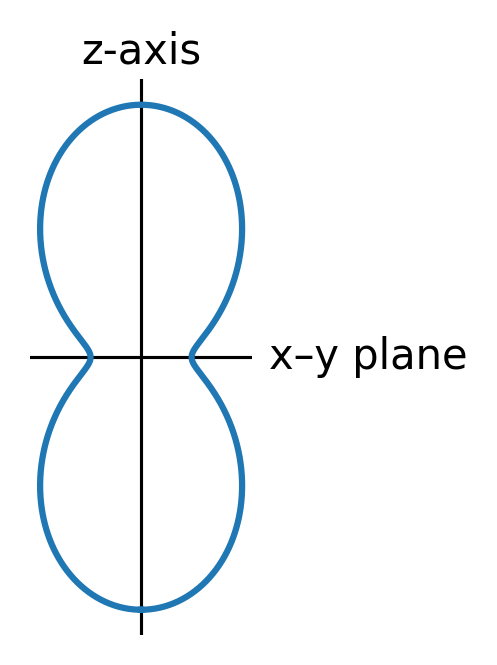
\includegraphics[width=4cm]{theory_of_gravitational_waves/images/cbc_quadrupole/radiation_pattern}
	\caption{Radiation pattern of a CBC system in the x--y plane visualized by plotting $g(\theta)\,(\cos\theta,\,\sin\theta)$} 
	\label{fig:gravitational_waves:radiation_pattern}
	% \vspace{-10pt}
\end{wrapfigure}

%\begin{equation}
%	P = -\frac{32}{5}\frac{c^5}{G}\left(\frac{G\pazocal{M}\pi f}{c^3}\right)^\frac{10}{3}
%\end{equation}
It can be shown that the radiated power per unit solid angle takes on the following form: 
\begin{equation}
	\frac{\mathrm{d}P}{\mathrm{d}\Omega} = \frac{2}{\pi}\frac{c^5}{G}\left(\frac{G\pazocal{M} \omega}{c^3}\right)^\frac{10}{3}g(\theta)
\end{equation}
with an angular distribution $g(\theta) = (1+\cos^2\theta)^2/4 + \cos^2\theta$.
(For further information consult \cite{10.1093/acprof:oso/9780198570745.001.0001}.)
This reveals that the radiated power scales with the orbital angular frequency $\omega^{10/3}$ and that most of that power is radiated along the z-axis, \emph{i.e.}\ perpendicular to the orbital plane (see Fig.~\ref{fig:gravitational_waves:radiation_pattern}). Now, the dependence on the frequency creates this feedback loop where the system continuously loses energy, which in turn decreases the orbital radius and increases the frequency leading to higher energy loss. This process gives rise to the characteristic chirp-like signal that is associated with CBCs, where up until the merger, the GW frequency and amplitude increase.

\begin{figure}
	\centering
	\makebox[\textwidth]{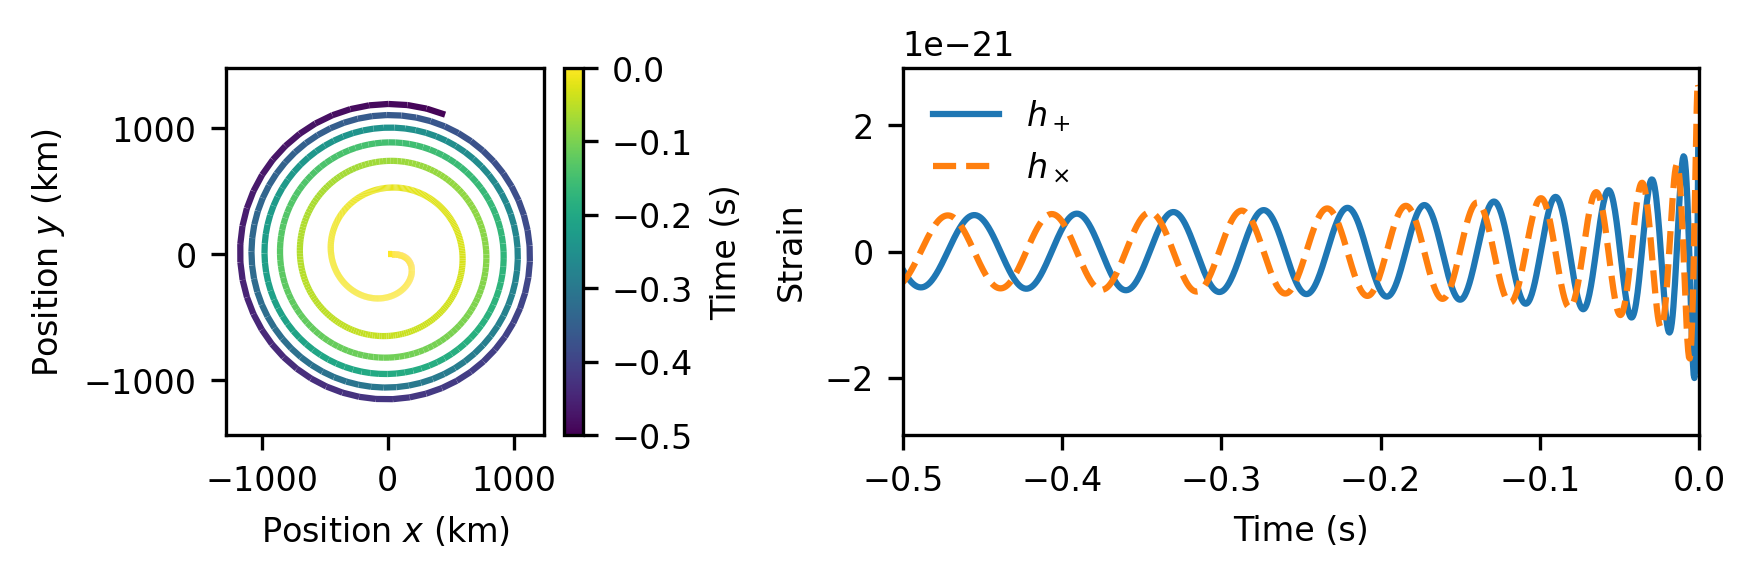
\includegraphics[width=15cm]{theory_of_gravitational_waves/images/coalescences/waveform}}
	\caption{Evolution of a CBC system. Trajectory of the reduced mass in the orbital plane in the center-of-mass frame on the left. The two polarizations of the emitted GW on the right.}
	\label{fig:gravitational_waves:waveform}
\end{figure}	
The evolution of $\omega(t)$ can be calculated by considering that the total energy of this system is $E = -Gm_1m_2/2R$. Equating $P$ and $-\mathrm{d}E/\mathrm{d}t$ results in a differential equation for $\omega$. Solving with respect to $\tau = t_\text{coa} - t$, the time to coalesce, yields
\begin{equation}
	\label{eq:gravitational_waves:cbc_freq}
	\omega(\tau) = \left(\frac{c^3}{G\pazocal{M}}\right)^\frac{5}{8}
	\left(\frac{5}{256}\frac{1}{\tau}\right)^\frac{3}{8}.
\end{equation}
With this result, the one-body motion in the center-of-mass frame can be obtained via Eq.~\ref{eq:gravitational_waves:cbc_pos} as well as the resulting GW waveform from Eq.~\ref{eq:gravitational_waves:cbc_waveform}. The dynamics of two inspiraling masses, \SI{40}{\solarmass} and \SI{30}{\solarmass}, and the emitted GW signal as measured at a distance of $r=\SI{500}{\mega\parsec}$ are plotted in Fig.~\ref{fig:gravitational_waves:waveform}. It can be seen in the last \SI{0.5}{\second}, the objects are very compact being separated by  $\pazocal{O}(\SI{100}{\kilo\meter})$. The corresponding signal is chirp-like and of order $\pazocal{O}(\SI{E-21})$, so very faint despite the large masses.

Observe that formally, the frequency diverges at the time of coalescence (Eq.~\ref{eq:gravitational_waves:cbc_freq}), which is of course unphysical. This divergence stems from the fact that the two objects get arbitrarily close. Realistically, the innermost stable orbit would be $r_\text{ISCO} = 6GM/c^2$, which corresponds to an angular orbital frequency of $\omega_\text{ISCO} = c^3/6\sqrt{6} GM$. This can be related to the emitted GW signal frequency as
\begin{equation}
	\label{eq:theory_of_gravitational_waves:max_freq_approx}
	f_\text{max} = \frac{\omega_\text{ISCO}}{\pi} 
	\approx \SI{4.4}{\kilo\hertz}\,\frac{\SI{1}{\solarmass}}{M}.
\end{equation}
For black hole binaries with masses $\pazocal{O}(\SI{10}{\solarmass})$ this means maximum frequencies of $\pazocal{O}(\SI{100}{\hertz})$ while neutron star binaries have masses $\approx\SI{1}{\solarmass}$ resulting in frequencies up to $\approx\SI{2000}{\hertz}$.
